\documentclass[12pt]{article}


% -------------------- PAQUETES --------------------
\usepackage[utf8]{inputenc}
\usepackage[spanish]{babel}
\usepackage[margin=2.54cm]{geometry}
\usepackage{graphicx}
\usepackage{xcolor}
\usepackage{enumitem}
\usepackage{parskip}
\usepackage{hyperref}
\usepackage{ulem} 
\usepackage{subcaption}


% -------------------- CARGA DE ARCHIVOS EXTERNOS --------------------
% ----------------- UTILIDADES PARA DAR UN MEJOR FORMATO DE DOCUMENTO -----------------  


\definecolor{azul}{rgb}{0.0039, 0.3098, 0.6196}


% Formato para el indice general ...........
\makeatletter
    \renewcommand{\@dotsep}{1.5}
    \renewcommand{\l@section}{\@dottedtocline{1}{1.5em}{2.3em}}
    \renewcommand{\l@subsection}{\@dottedtocline{2}{3.8em}{3.2em}}
    \renewcommand{\l@subsubsection}{\@dottedtocline{3}{7.0em}{4.1em}}
\makeatother

% --------- COMANDOS PERSONALIZADOS PARA LA PORTADA DE LAS TAREAS, TRABAJOS Y PROYECTOS ---------

\newcommand{\rutaLogo}[1]{\newcommand{\RutaLogo}{#1}}
\newcommand{\tema}[1]{\newcommand{\Tema}{#1}}
\newcommand{\etiquetaAutores}[1]{\newcommand{\EtiquetaAutores}{#1}}
\newcommand{\alumno}[1]{\newcommand{\Alumno}{#1}}
\newcommand{\materia}[1]{\newcommand{\Materia}{#1}}
\newcommand{\docente}[1]{\newcommand{\Docente}{#1}}
\newcommand{\ciclo}[1]{\newcommand{\Ciclo}{#1}}
\newcommand{\fecha}[1]{\newcommand{\Fecha}{#1}}
\newcommand{\periodo}[1]{\newcommand{\Periodo}{#1}}



% -------------------- DEFINICIÓN DE LA PORTADA --------------------
\rutaLogo{../../../../docs/img/logo-ista.png}
\tema{\\ \vspace{0.5cm} Guía Práctica N°1 - Captura y adquisición de datos \\ \vspace{1.2cm}}
\etiquetaAutores{Integrantes:}
\alumno{Eduardo Mendieta\\Freddy Montalván\vspace{0.7cm}}
\materia{Introducción a Big Data \vspace{0.7cm}}
\docente{MSc. Ing. Carmen Tacuri Vintimilla \vspace{0.7cm}}
\ciclo{Primer Ciclo \vspace{0.7cm}}
\fecha{29 de julio de 2024 \vspace{0.7cm}}
\periodo{Abril 2024 - Agosto 2024}

\begin{document}

        \begin{titlepage}

    \centering

    \includegraphics[width=0.11\textwidth]{\RutaLogo} 

    \vspace{0.3cm}
    \textcolor{azul}{\Large \textbf{Instituto Superior Universitario Tecnológico del Azuay \\}}
    \vspace{0.3cm}
    \textcolor{azul}{\Large \textbf{Tecnología Superior en Big Data}}
    
    % 1. ---------------- TEMA -------------------------
    
    {\Large\textbf{\Tema}}
    
    % 2. ---------------- AUTOR(ES) -------------------------
    \textcolor{azul}{\large \textbf{\EtiquetaAutores} \\}
    \vspace{0.3cm}
    {\large \Alumno}

    % 3. ---------------- MATERIA -------------------------
    \textcolor{azul}{\large \textbf{Materia:} \\}
    \vspace{0.3cm}
    {\large \Materia}


    % 3. ---------------- DOCENTE -------------------------
    \textcolor{azul}{\large \textbf{Docente:} \\}
    \vspace{0.3cm}
    {\large \Docente}


    % 3. ---------------- Ciclo -------------------------
    \textcolor{azul}{\large \textbf{Ciclo:} \\}
    \vspace{0.3cm}
    {\large \Ciclo}


    % 3. ---------------- FECHA -------------------------
    \textcolor{azul}{\large \textbf{Fecha:} \\}
    \vspace{0.3cm}
    {\large \Fecha}

    % 3. ---------------- PERIODO -------------------------
    \textcolor{azul}{\large \textbf{Periodo Académico:} \\}
    \vspace{0.3cm}
    {\large \Periodo}
 
\end{titlepage}


        \tableofcontents
        \newpage

        \section*{\centering Guía Práctica N°1 - Captura y adquisición de datos}

        % 1.Introducción: ...................................................
        \section{Introducción}
        En el análisis de datos, la captura y adquisición de datos juegan un papel crucial al proporcionar la base sobre la cual se construyen los insights y las decisiones informadas. Estos procesos comprenden la identificación, recolección e integración de información relevante, que puede provenir de una variedad de fuentes, como sistemas, sensores, encuestas o archivos. La captura se enfoca en recoger datos brutos, mientras que la adquisición se centra en organizar y almacenar estos datos para su procesamiento posterior.

        Una técnica destacada en la captura y adquisición de datos es el web scraping, que permite la extracción automatizada de información de sitios web. Utilizando scripts o herramientas especializadas, el web scraping facilita la obtención de datos específicos de páginas web, incluso cuando estos datos no están disponibles en formatos estructurados o accesibles. Esta técnica resulta invaluable para recolectar grandes volúmenes de información de manera eficiente, facilitando así el análisis de tendencias, la investigación de mercado y la toma de decisiones basada en datos actualizados.

        Entre las herramientas más útiles para el web scraping se encuentra IMPORTHTML en Google Sheets, que permite importar tablas o listas desde páginas web y mantener los datos actualizados automáticamente. Adicionalmente, Table Capture es una extensión para Chrome que simplifica la extracción de datos de tablas HTML y su exportación a formatos como Google Sheets, Excel o CSV. Para extraer datos de tablas en archivos PDF, Tabula es una aplicación de escritorio compatible con múltiples sistemas operativos que convierte estos datos en formatos editables como CSV o Excel. Hunter.io, por su parte, se especializa en la recopilación de correos electrónicos de sitios web, facilitando la ampliación de listas de contactos. Finalmente, Octoparse es una herramienta de web scraping intuitiva y con una prueba gratuita, que permite a usuarios sin experiencia en programación extraer datos de cualquier sitio web con facilidad y exportarlos en diversos formatos.

        Estas herramientas y técnicas son fundamentales para realizar una captura y adquisición de datos efectiva, asegurando que la información recolectada sea precisa, completa y lista para su análisis y aplicación.
        

        % 2.Objetivos: ...................................................
        \newpage
        \section{Objetivos}
                \subsection{Objetivo general}
                        Explorar las herramientas de scraping presentadas en la guía, adquiriendo un conocimiento básico sobre su uso para la captura y adquisición de datos.

                \subsection{Objetivos específicos}
                        \begin{itemize}
                        \item Extraer los datos de la web oficial con información actual sobre el COVID-19 utilizando las herramientas propuestas en la guía.
                        \item Examinar las interfaces que ofrecen cada una de estas aplicaciones y extensiones para la captura de datos.
                        \item Concluir sobre las ventajas, similitudes y diferencias entre estas herramientas.
                        \end{itemize}


        % 3.Paso a Paso: ...................................................
        \newpage
        \section{Paso a paso}
                \subsection{Fórmula ImportHTML}
                        En Google Sheets, la función \textit{IMPORTHTML} permite importar tablas o listas desde páginas web externas, actualizando automáticamente los datos en la hoja de cálculo cuando se realizan cambios en la fuente original. La sintaxis de la función es \textit{=IMPORTHTML(url, consulta, índice)}, donde \textit{url} es la dirección del sitio web, \textit{consulta} especifica si se desea importar una tabla o una lista, y \textit{índice} indica el número de la tabla o lista a importar. 
                        
                        Por ejemplo, para extraer datos estadísticos del Covid-19 de una página específica, se puede usar la fórmula \textit{=IMPORTHTML(\href{https://www.coronavirusecuador.com/datos-provinciales/}{"https://www.coronavirusecuador.com/datos-provinciales"}; table" ;1)} para capturar la primera tabla disponible en la web, y los datos se mostrarán automáticamente en la hoja de cálculo.

                        \begin{figure}[!h]
                                \centering
                                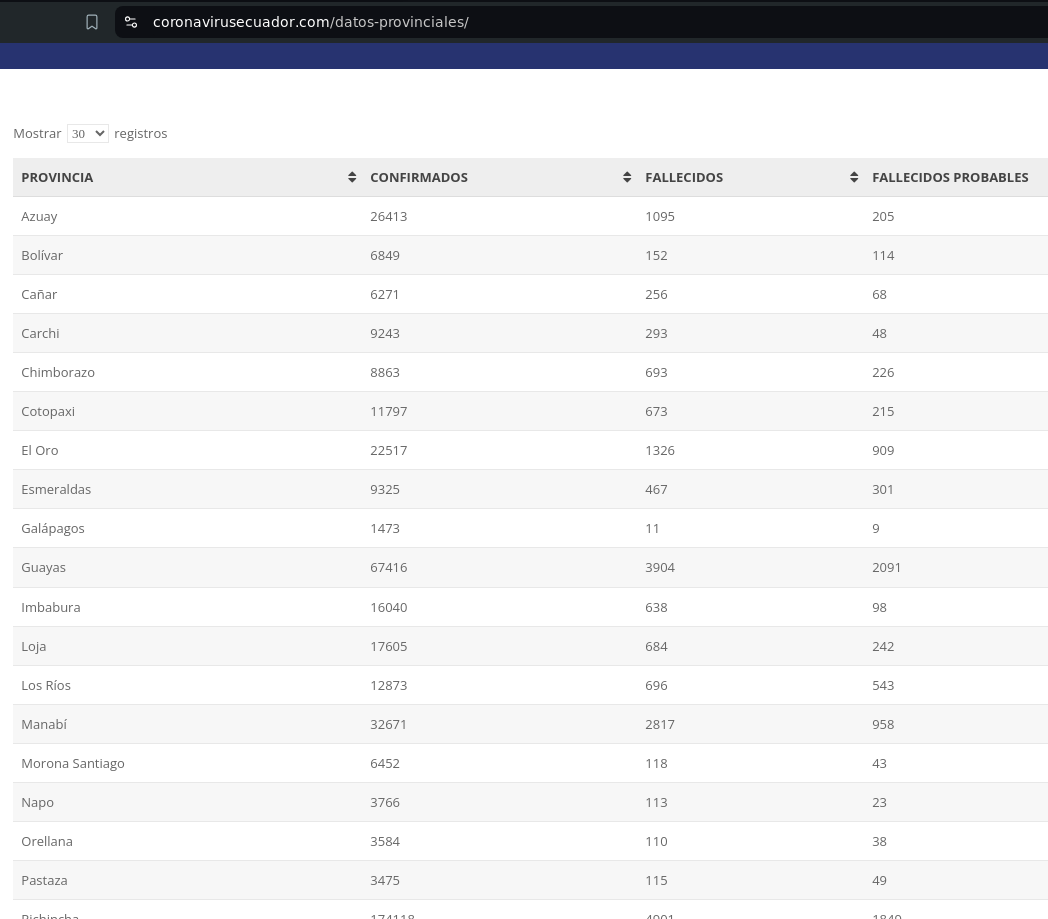
\includegraphics[width=0.9\textwidth]{img/importhtml-1.png}
                                \caption{Datos estadísticos del Covid- 19}
                        \end{figure}

                        \newpage
                        \begin{figure}[!h]
                                \centering
                                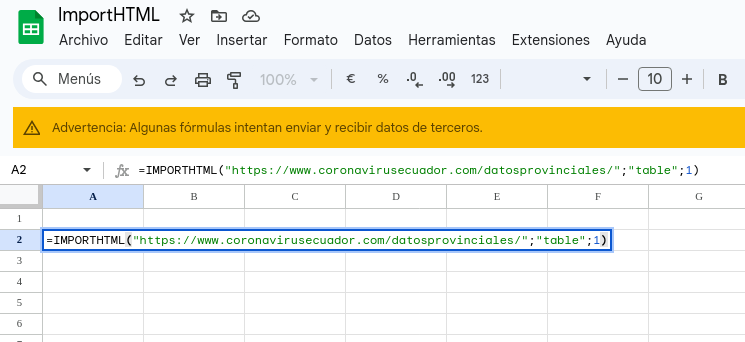
\includegraphics[width=0.7\textwidth]{img/importhtml-2.png}
                                \caption{Fórmula para importar los datos del Covid- 19 en la hoja de cálculo de Google}
                        \end{figure}

                        \begin{figure}[!h]
                                \centering
                                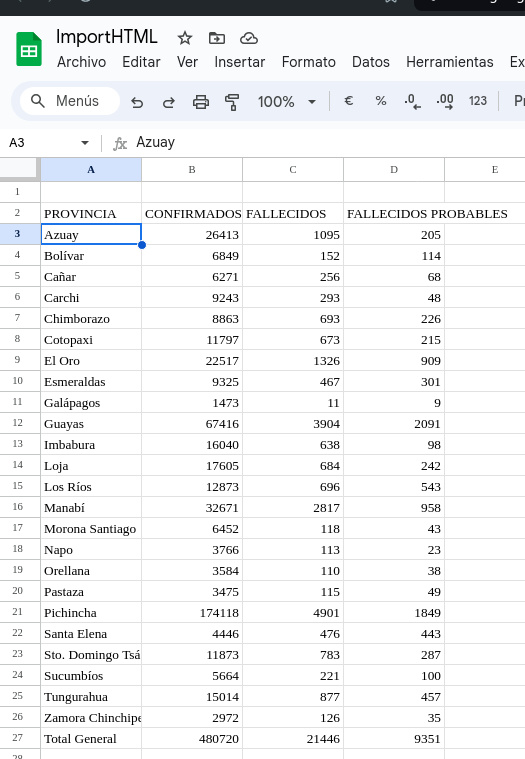
\includegraphics[width=0.6\textwidth]{img/importhtml-3.png}
                                \caption{Datos importados en la hoja de cálculo de Google}
                        \end{figure}

                \subsection{Table capture}
                        Table Capture es una extensión para el navegador Chrome que facilita la extracción de datos de tablas HTML en páginas web, permitiendo su exportación a formatos como Google Sheets, Excel o CSV, similar a la función \textit{IMPORTHTML}. 
                        
                        Tras instalar la extensión y acceder a la página de datos del Covid-19 en Ecuador, se puede utilizar la opción \textit{Captura de tabla} del menú contextual para copiar la información al portapapeles o abrirla directamente en Google Sheets. Aunque las funciones avanzadas de exportación y almacenamiento en la nube están disponibles solo en la versión Pro, la versión gratuita permite copiar y modificar los datos antes de su uso.
                        
                        \begin{figure}[!h]
                                \centering
                                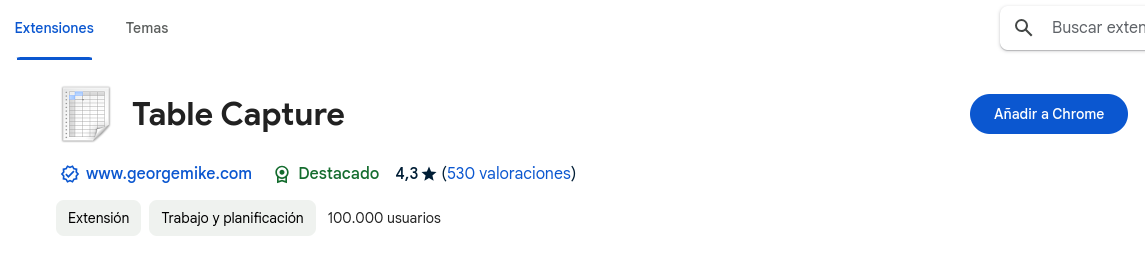
\includegraphics[width=1\textwidth]{img/tablecapture-1.png}
                                \caption{Añadiendo Table Capture a Chrome}
                        \end{figure}

                        \begin{figure}[!h]
                                \centering
                                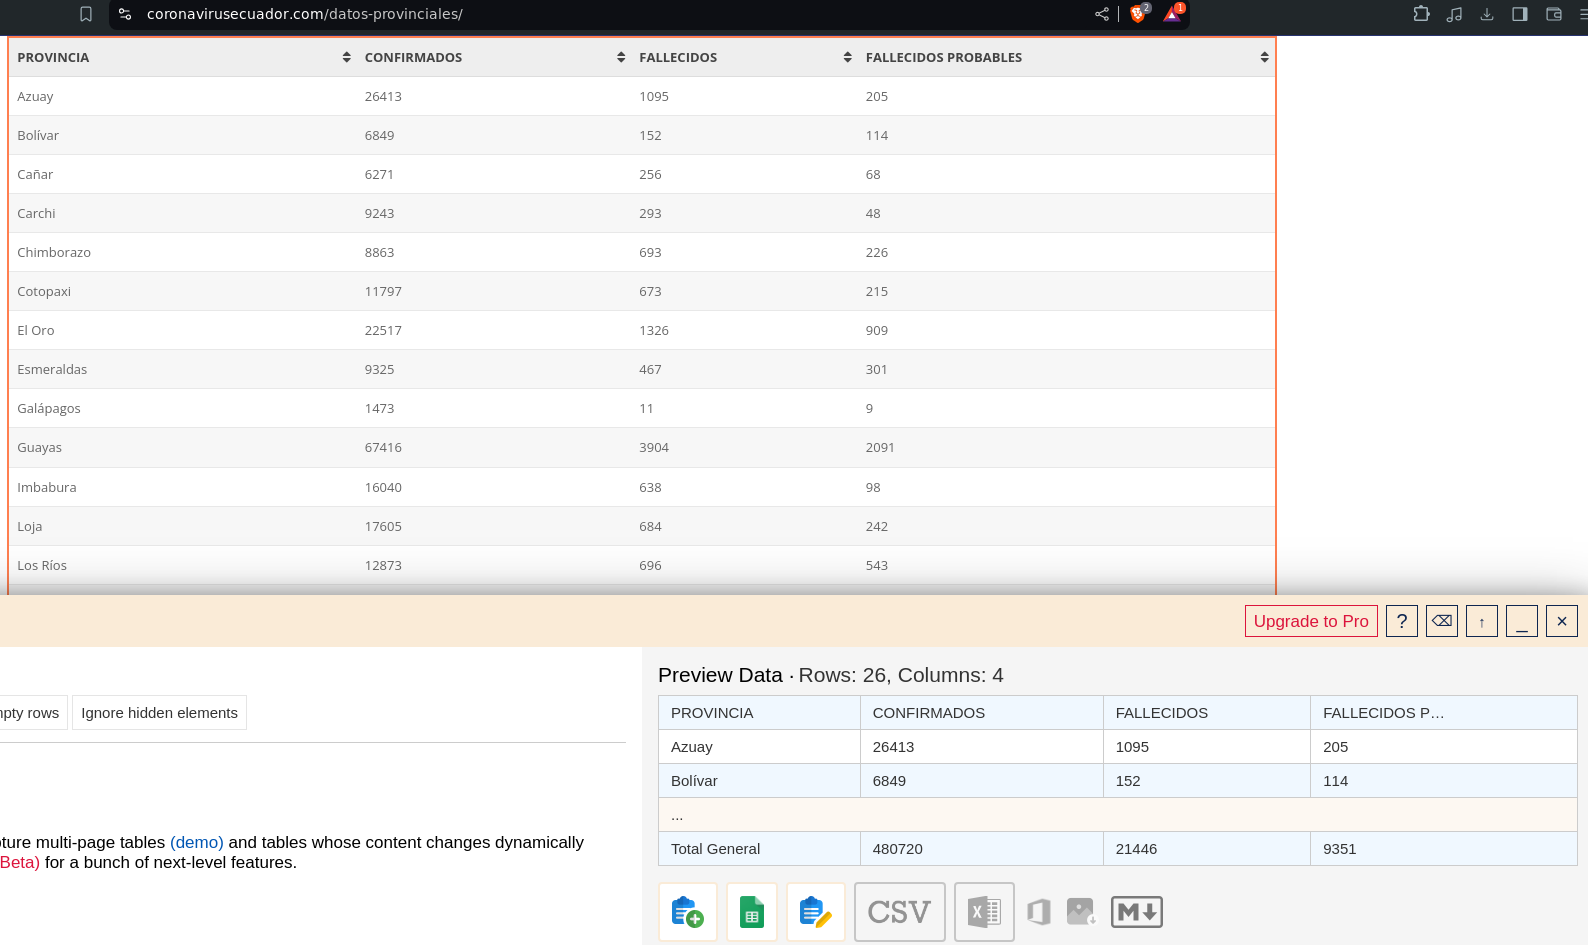
\includegraphics[width=0.9\textwidth]{img/tablecapture-2.png}
                                \caption{Seleccionando los datos y exportando a una hoja de cálculo de Google}
                        \end{figure}

                        \newpage
                        \begin{figure}[!h]
                                \centering
                                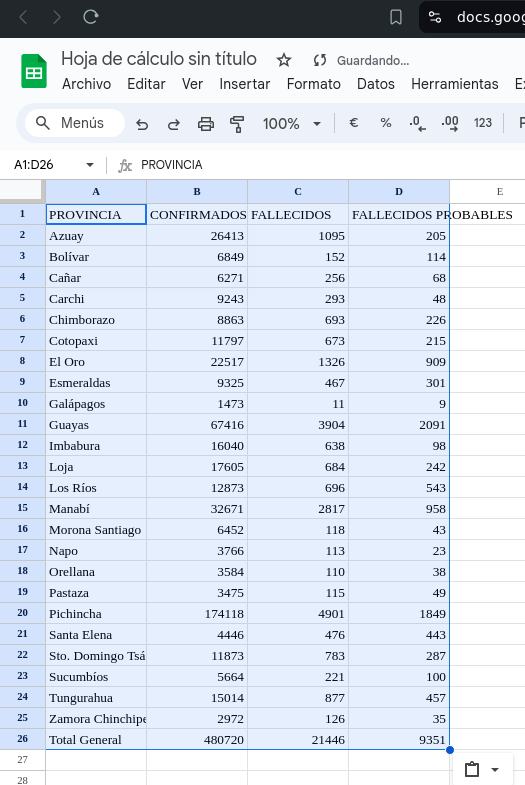
\includegraphics[width=0.6\textwidth]{img/tablecapture-3.png}
                                \caption{Pegando los datos obtenidos con Table Capture}
                        \end{figure}

                \subsection{Tabula}
                        Tabula es una aplicación de escritorio compatible con Windows, Mac OSX y Linux, que simplifica la extracción de datos de tablas en archivos PDF a formatos editables como CSV o Microsoft Excel, siendo especialmente útil en el periodismo de datos. Para instalarla, se debe descargar el archivo correspondiente desde \href{https://tabula.technology/ }{\uline{su pagina web oficial}}, seguir las instrucciones específicas según el sistema operativo. Tras la instalación, se carga el archivo PDF con la tabla deseada en Tabula, se usa la opción \textit{Autodetect Tables} para identificar y extraer los datos, y se puede revisar la información extraída antes de exportarla a un archivo CSV o Excel. La aplicación permite también la visualización y modificación de los datos antes de su exportación.

                        \newpage
                        \begin{figure}[!h]
                                \centering
                                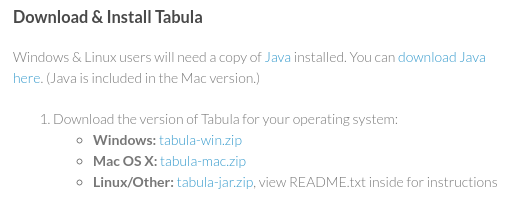
\includegraphics[width=1\textwidth]{img/tabula-1.png}
                                \caption{Descarga de Tabula}
                        \end{figure}

                        \begin{figure}[!h]
                                \centering
                                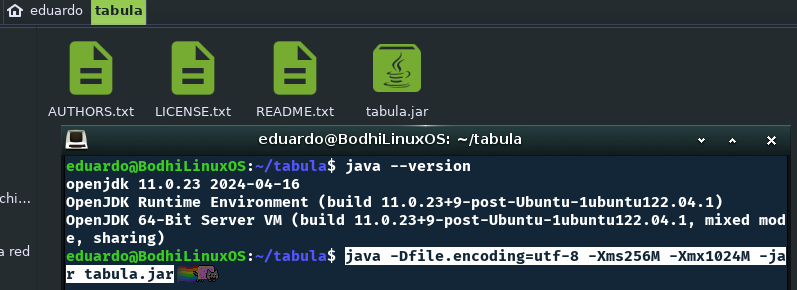
\includegraphics[width=1\textwidth]{img/tabula-2.png}
                                \caption{Ejecución de Tabula}
                        \end{figure}

                        \begin{figure}[!h]
                                \centering
                                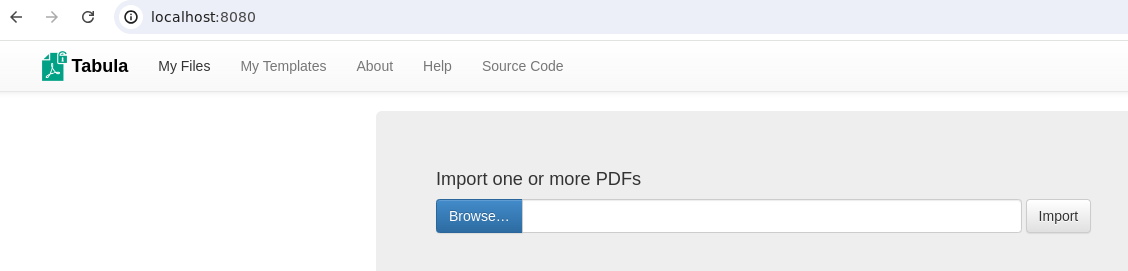
\includegraphics[width=1\textwidth]{img/tabula-3.png}
                                \caption{Importando PDF con datos sobre el Covid-19}
                        \end{figure}

                        \newpage
                        \begin{figure}[!h]
                                \centering
                                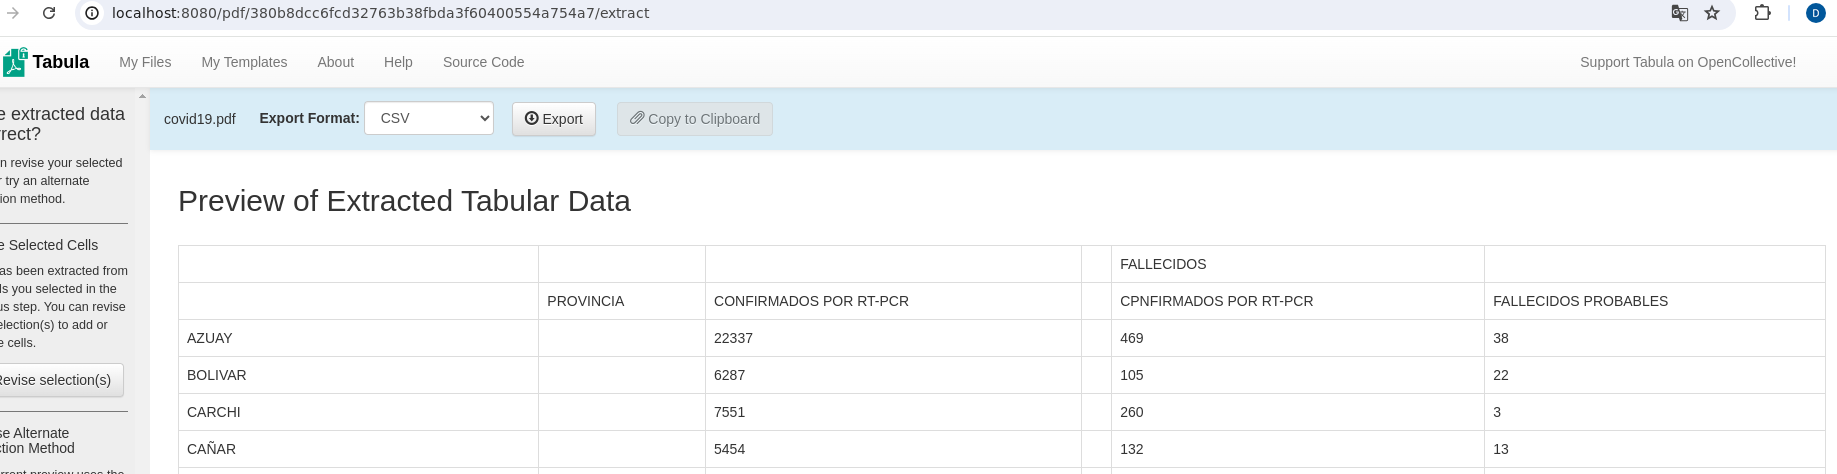
\includegraphics[width=1\textwidth]{img/tabula-4.png}
                                \caption{Extraendo los datos del PDF con Tabula}
                        \end{figure}

                        \begin{figure}[!h]
                                \centering
                                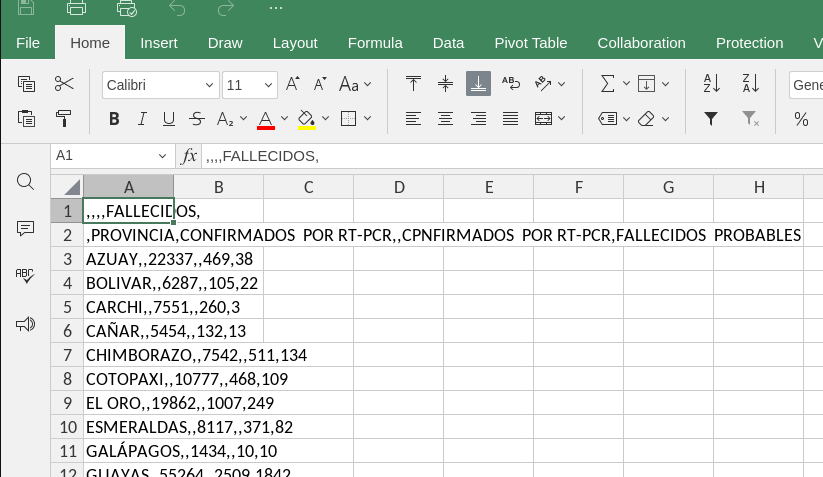
\includegraphics[width=1\textwidth]{img/tabula-5.png}
                                \caption{Datos importados en formato CSV}
                        \end{figure}

                \subsection{Hunter.io}
                        \textit{Hunter.io} es una herramienta en línea diseñada para la recopilación de correos electrónicos a partir de sitios web, funcionando como un buscador especializado en encontrar direcciones de correo electrónico. Ideal para ampliar listas de contactos empresariales y realizar campañas de marketing por correo, \textit{Hunter.io} permite buscar emails asociados a un dominio específico, como \textit{colinealcorp.com}. Al ingresar el dominio, se muestra una lista de correos electrónicos encontrados en la web, con detalles adicionales disponibles al hacer clic en cada ítem. Aunque el uso básico es anónimo y gratuito, también es posible crear una cuenta para exportar los datos en formato CSV y acceder a funcionalidades adicionales.
                        
                        \begin{figure}[!h]
                                \centering
                                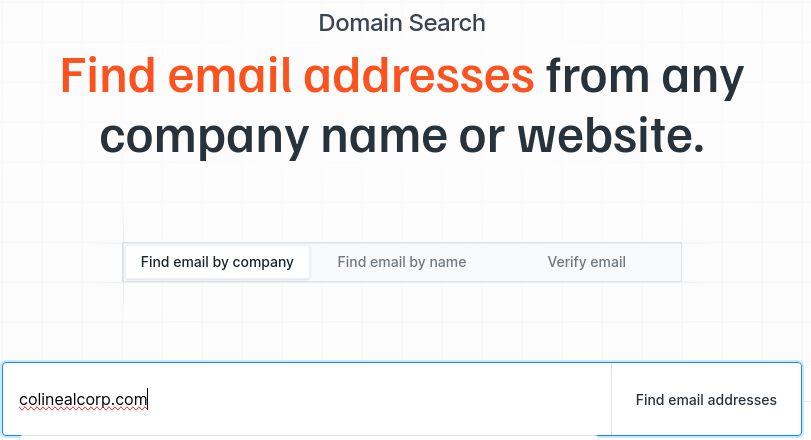
\includegraphics[width=1\textwidth]{img/hunter-1.png}
                                \caption{Buscando el dominio \textit{colinealcorp.com}}
                        \end{figure}

                        \begin{figure}[!h]
                                \centering
                                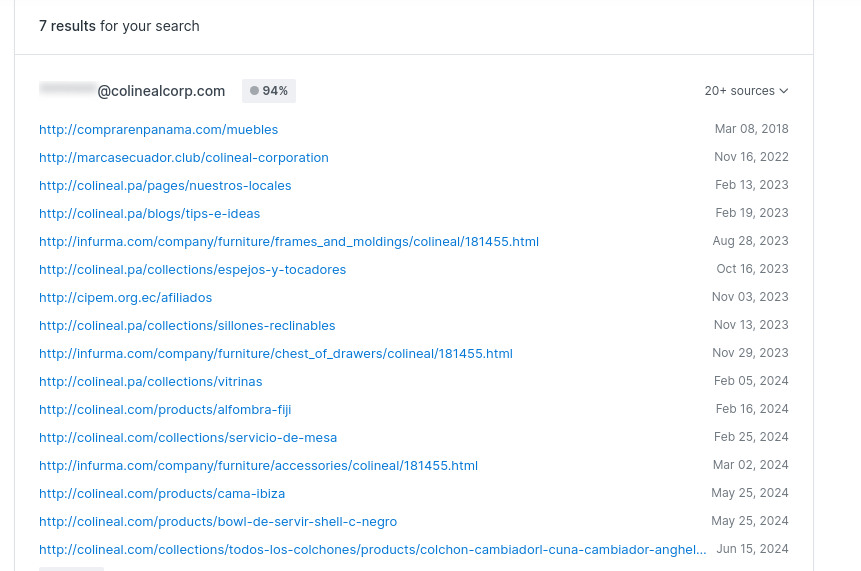
\includegraphics[width=1\textwidth]{img/hunter-2.png}
                                \caption{lista de correos asociados al domino}
                        \end{figure}

                        \begin{figure}[!h]
                                \centering
                                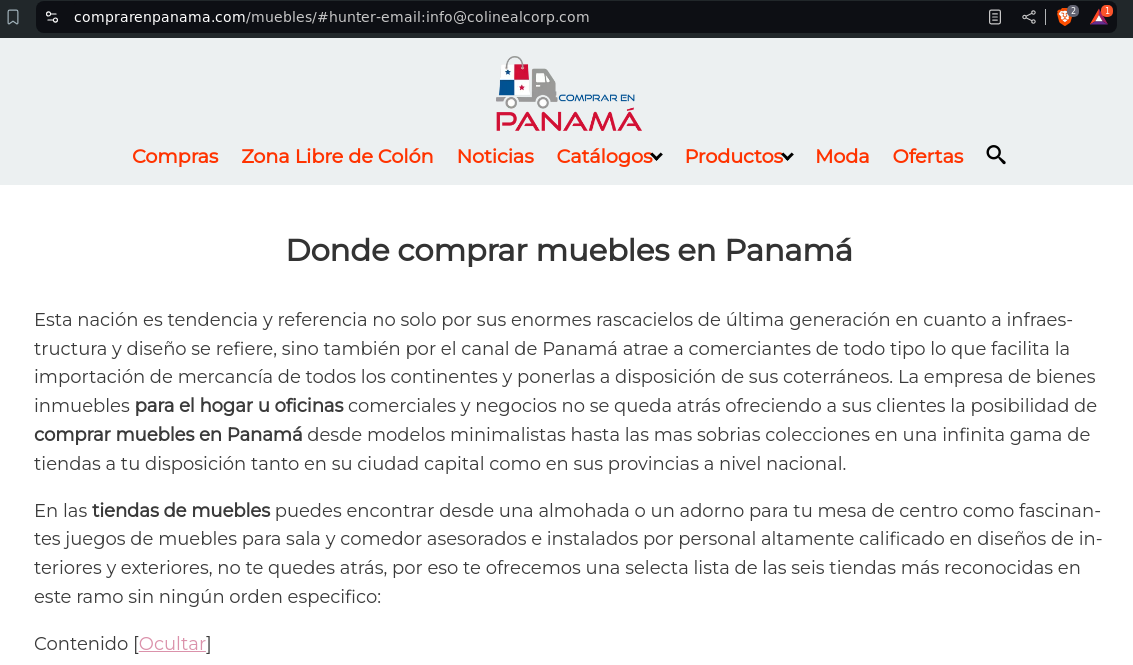
\includegraphics[width=1\textwidth]{img/hunter-3.png}
                                \caption{Desplegando uno de los items}
                        \end{figure}
                
                \subsection{Octoparse}
                        Octoparse es una herramienta de web scraping gratuita y fácil de usar, diseñada para usuarios sin experiencia en programación. Permite extraer datos de cualquier sitio web mediante su función de detección automática, evitando los complicados procesos de construcción de crawlers. Los datos extraídos pueden exportarse en formatos como Excel, CSV, JSON, HTML, o a bases de datos. Para utilizar Octoparse, se debe registrar una cuenta en su página web y descargar el cliente de escritorio desde un archivo comprimido. 
                        
                        Tras la instalación, se accede con las credenciales registradas y se pueden usar plantillas predefinidas o personalizadas para capturar datos de diversas fuentes, como Google Search. Al ejecutar una búsqueda, como sobre el Covid-19 en Ecuador, la aplicación realiza la extracción y permite exportar los datos obtenidos. Aunque la prueba gratuita requiere una tarjeta de crédito, la guía permite comprender el funcionamiento de la herramienta sin problemas.

                        \newpage
                        \begin{figure}[!h]
                                \centering
                                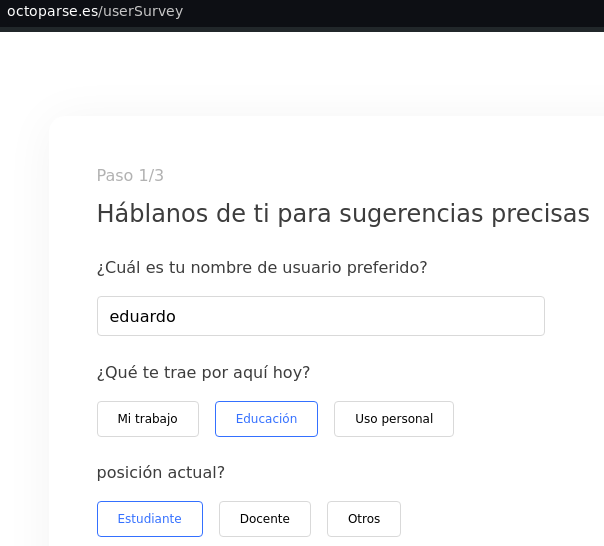
\includegraphics[width=0.8\textwidth]{img/octoparse-1.png}
                                \caption{Creando una cuenta gratuita en Octoparse}
                        \end{figure}
                        \begin{figure}[!h]
                                \centering
                                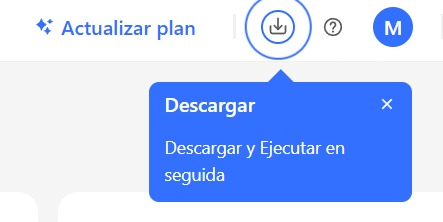
\includegraphics[width=0.6\textwidth]{img/octoparse-2.png}
                                \caption{Descarga de la aplicación de escritorio}
                        \end{figure}
                        \newpage
                        \begin{figure}[!h]
                                \centering
                                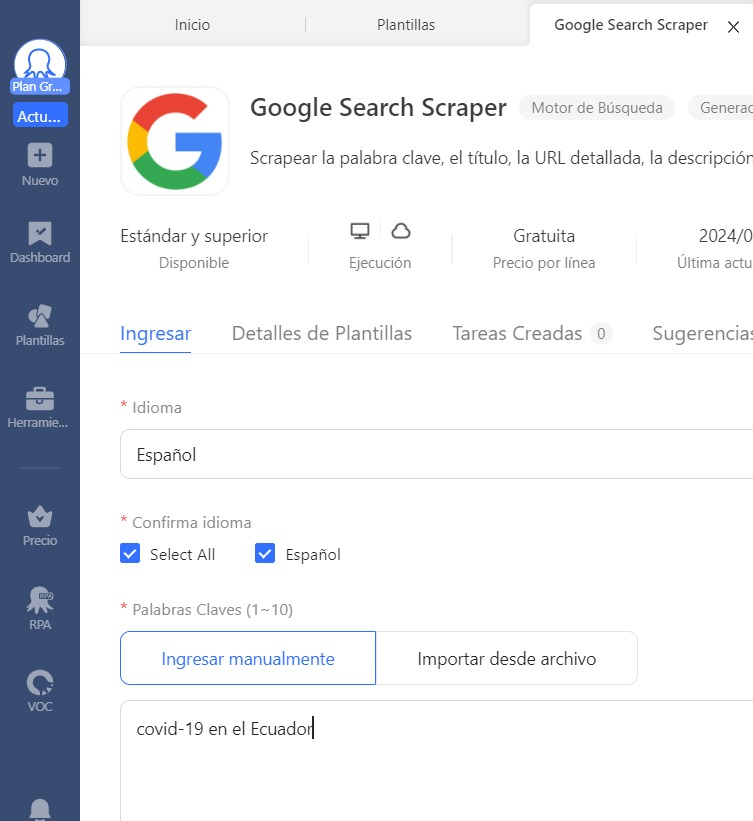
\includegraphics[width=0.8\textwidth]{img/octoparse-3.png}
                                \caption{Seleccionando el motor de búsqueda}
                        \end{figure}
                        \begin{figure}[!h]
                                \centering
                                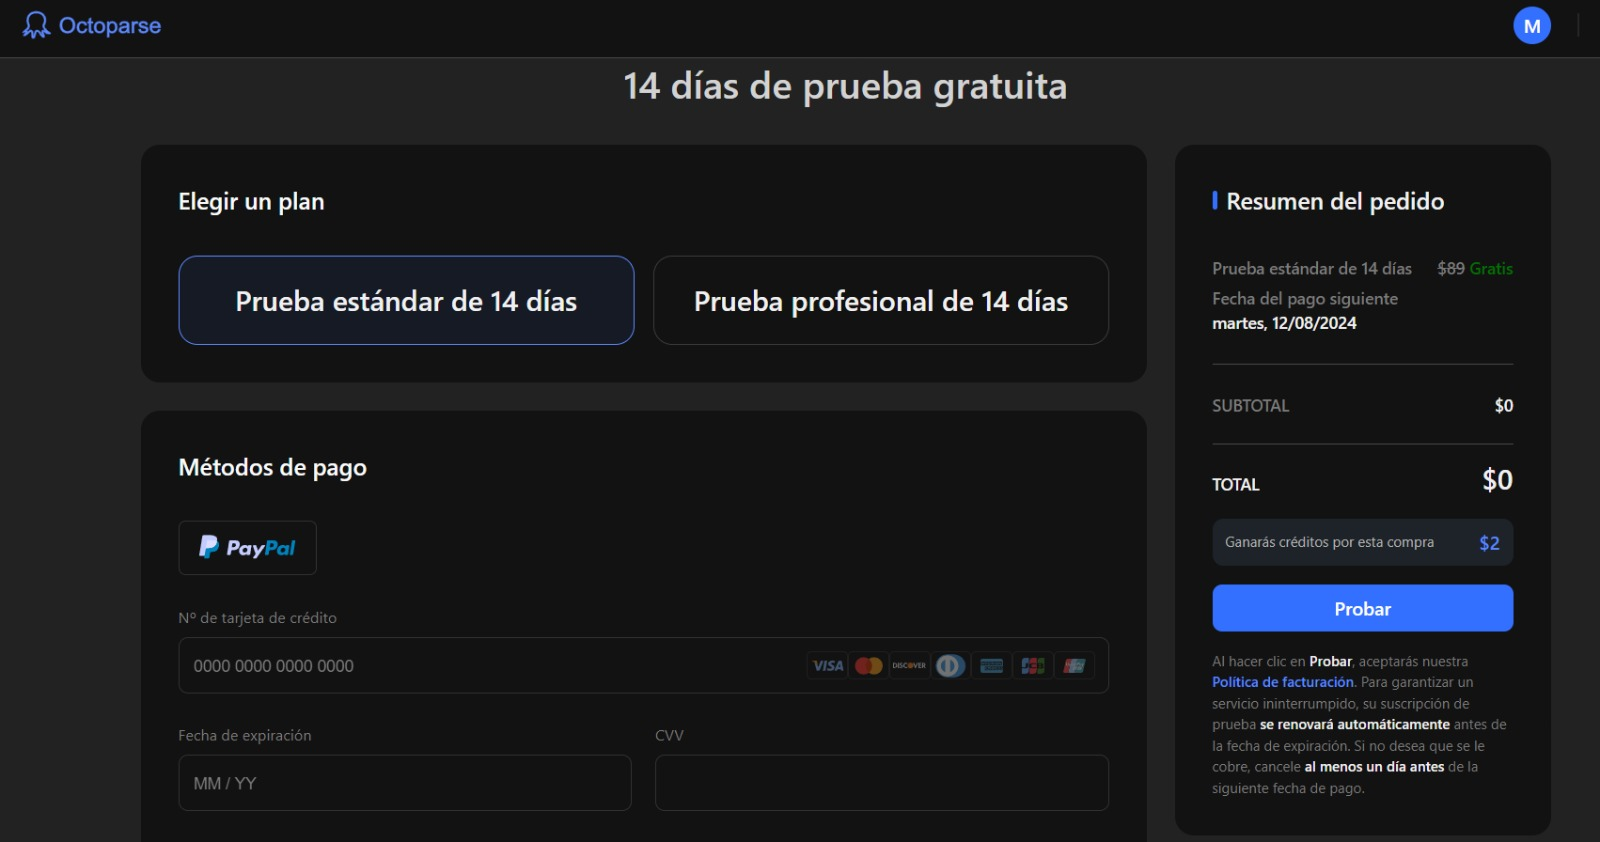
\includegraphics[width=0.6\textwidth]{img/octoparse-4.png}
                                \caption{Solicitu de ingreso de tarjeta}
                        \end{figure}


        % 4.Conclusiones: ...................................................
        \newpage
        \section{Conclusiones y recomendaciones}
                \subsection{Conclusiones}
                        \begin{enumerate}
                                \item La función IMPORTHTML de Google Sheets permite importar y actualizar automáticamente datos de tablas o listas desde páginas web, integrando los datos directamente en una hoja de cálculo sin necesidad de herramientas adicionales. Esta función es ideal para usuarios que desean mantener los datos sincronizados con la fuente web en tiempo real, facilitando el análisis y la visualización de información directamente dentro de Google Sheets.
                                \item Table Capture, como extensión para el navegador Chrome, ofrece una forma sencilla de copiar datos de tablas visibles en páginas web y exportarlos a formatos como Google Sheets, Excel o CSV. Aunque la versión gratuita proporciona funcionalidades básicas, la versión Pro amplía las opciones y soporta características avanzadas. Esta herramienta es útil para usuarios que prefieren una solución rápida y directa para capturar datos desde la web sin tener que realizar configuraciones complejas.
                                \item Por otro lado, Tabula está diseñada específicamente para extraer datos de tablas dentro de archivos PDF, convirtiéndolos en formatos editables como CSV o Excel. A diferencia de las otras herramientas mencionadas, Tabula trabaja con documentos locales en lugar de datos web, lo que la hace esencial para quienes necesitan transformar contenido de PDF en datos estructurados para su análisis o procesamiento.
                                \item Hunter.io se centra en la búsqueda y recopilación de correos electrónicos desde sitios web, facilitando la creación de listas de contactos para marketing y otras aplicaciones. Mientras que la funcionalidad básica es gratuita, las características más avanzadas y la capacidad para exportar datos requieren una suscripción paga. Es una herramienta especializada para quienes buscan expandir y gestionar listas de contactos empresariales a partir de información disponible en la web.
                                \item Finalmente, Octoparse proporciona una solución completa para el web scraping, permitiendo la extracción de datos de cualquier sitio web y exportándolos en diversos formatos como Excel, CSV, JSON o bases de datos. Su interfaz amigable y capacidades de detección automática la hacen accesible para usuarios sin experiencia en programación. Sin embargo, la versión gratuita puede estar limitada en cuanto a funcionalidades y puede requerir una tarjeta de crédito para pruebas extensivas, lo que la diferencia de otras herramientas más simples o específicas.
                        \end{enumerate}

                \subsection{Recomendaciones}
                        \begin{enumerate}
                                \item Como única recomendación, se sugiere buscar herramientas de código abierto como alternativas a algunas de las herramientas propuestas en la guía, ya que estas pueden tener limitaciones en comparación con sus versiones de pago.
                        \end{enumerate}


        % 5.Bibliografía: ...................................................
        \section{Bibliografía}
                \begin{itemize}
                        \item Guía practica proporcionada por la docente. 
                \end{itemize}


\end{document}